There are multiple ways to approach discretizing the ellipse, the most apparent of which being
\begin{equation}\label{eq:parametric_ellipse}
  \xtt = a\cos{t} + b\sin{t}, \qquad t \in [0, 2\pi),
\end{equation}
where the parameter is \emph{not} a polar variable.
It is indeed related, as will be shown.
\begin{Figure}
  \centering
  \scalebox{1}{%
    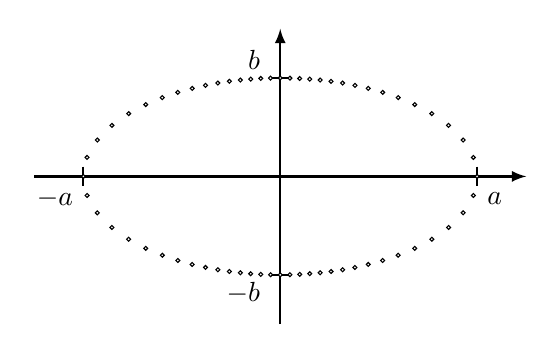
\begin{tikzpicture}
  \begin{scope}[scale = 2.5]
    \def\majradius{1}
    \def\minradius{0.5}
    \def\slingringsmonn{.25}
    \draw[-latex, thick] ({-\majradius - \slingringsmonn}, 0)--({\majradius + \slingringsmonn}, 0);
    \draw[-latex, thick] (0, {-\minradius - \slingringsmonn})--(0, {\minradius + \slingringsmonn});
    \draw[thick] ({-\majradius}, .05)--({-\majradius}, -.05) node[below = 1ex, left]{$-a$};
    \draw[thick] ({\majradius}, .05)--({\majradius}, -.05) node[below = 1ex, right]{$a$};
    \draw[thick] (.05, {\minradius})--(-.05, {\minradius}) node[above = 1.5ex, left]{$b$};
    \draw[thick] (.05, {-\minradius})--(-.05, {-\minradius}) node[below = 1.5ex, left]{$-b$};
    \def\numbernodes{64}
    \foreach \i in {0, ..., \numbernodes}
      \pgfmathsetmacro\teta{2 *\i * pi / \numbernodes}
      \def\radius{(\majradius*\minradius)/sqrt(\minradius^2 * (cos(\teta r))^2 + \majradius^2 * (sin(\teta r))^2)}
      \draw[fill = white] ({\radius*cos(\teta r)}, {\radius*sin(\teta r)}) circle (.01);
  \end{scope}
\end{tikzpicture}

  }
  \captionsetup{type = figure}
  \caption{Ellipse parametrized with equidistant spacing in the perimeter.}
\end{Figure}
\begin{Figure}
  \centering
  \scalebox{1}{%
    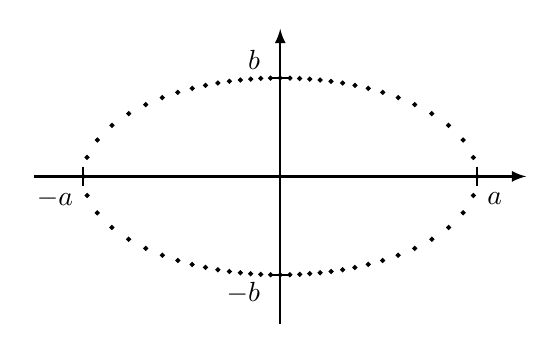
\begin{tikzpicture}
  \begin{scope}[scale = 2.5]
    \def\majradius{1}
    \def\minradius{0.5}
    \def\slingringsmonn{.25}
    \draw[-latex, thick] ({-\majradius - \slingringsmonn}, 0)--({\majradius + \slingringsmonn}, 0);
    \draw[-latex, thick] (0, {-\minradius - \slingringsmonn})--(0, {\minradius + \slingringsmonn});
    \draw[thick] ({-\majradius}, .05)--({-\majradius}, -.05) node[below = 1ex, left]{$-a$};
    \draw[thick] ({\majradius}, .05)--({\majradius}, -.05) node[below = 1ex, right]{$a$};
    \draw[thick] (.05, {\minradius})--(-.05, {\minradius}) node[above = 1.5ex, left]{$b$};
    \draw[thick] (.05, {-\minradius})--(-.05, {-\minradius}) node[below = 1.5ex, left]{$-b$};
    \def\numbernodes{64}
    \foreach \i in {0, ..., \numbernodes}
      \pgfmathsetmacro\teta{2 *\i * pi / \numbernodes}
      \def\radius{(\majradius*\minradius)/sqrt(\minradius^2 * (cos(\teta r))^2 + \majradius^2 * (sin(\teta r))^2)}
      \draw[fill = black] ({\radius*cos(\teta r)}, {\radius*sin(\teta r)}) circle (.01);
  \end{scope}
\end{tikzpicture}

  }
  \captionsetup{type = figure}
  \caption{Ellipse parametrized with equiangular spacing.}
\end{Figure}
